\section{Реализация}
\subsection{LSM-дерево}

LSM-дерево (log-structured merge-tree)  - это структура данных «ключ-значение» с хорошими характеристиками производительности. Это хороший выбор для обеспечения индексированного доступа к файлам данных, таким как данные журнала транзакций или данные временных рядов. Дерево LSM хранит данные в двух или более структурах. Каждая из них оптимизирована для конкретного типа памяти, на котором она хранится, а синхронизация между слоями выполняется поблочно~\cite{lsm_tree_orig}.

Простое дерево LSM состоит из двух уровней с именами $C_0$ и $C_1$. Основное различие между этими уровнями состоит в том, что обычно $C_0$ представляет собой структуру данных в оперативной памяти, а $C_1$ хранится на жестком диске. Следовательно, $C_1$ обычно больше, чем $C_0$, и когда объем данных в $C_0$ превышает некоторый предел, данные перемещаются в $C_1$. Чтобы поддерживать подходящую производительность, обычно рекомендуется оптимизировать как $C_0$, так и $C_1$ для конкретных условий применения. При этом данные рекомендуется переносить между слоями наиболее эффективно, возможно, с использованием алгоритмов, похожих на сортировку слиянием.

Для сохранения эффективности сохранения данных в уровне $C_1$, было решено использовать SSTable в качестве уровня $C_1$ и B-дерево для $C_0$. SSTable, или sorted string table - это файл, содержащий пары ключ-значение, отсортированные по ключу ~\cite {sstable}. Использование SSTable для хранения данных временных рядов обычно является хорошим решением, если данные передаются из системы мониторинга или даталоггинга. Из-за этого они сортируются по отметке времени, которая является хорошим кандидатом на ключ, значением же в SSTable может быть само измерение. SSTable всегда является неизменяемой структурой данных, что означает, что данные нельзя напрямую удалить из файла; измерения необходимо помечать «удаленными», а затем пропускать эти данные в процессе уплотнения SST-файла (compaction). Процесс уплотнения также используется для удаления устаревших данных, если для них предполагается определенный срок хранения (expiration).

\subsection{Журнал фиксации}
Любое приложение, которое используется для работы с критически важными данными, должно иметь возможность постоянного сохранения данных в случае отключения электроэнергии или любого другого неожиданного завершения работы приложения. Чтобы поддерживать эту возможность, используется механизм журнала фиксации (commitlog). Это доступный только для записи журнал любых вставок в базу данных. Он записывается перед добавлением данных в файлы данных базы данных. Этот механизм обычно используется в любых реляционных или не связанных СУБД.

Поскольку встраиваемая система хранения данных также должна поддерживать эту возможность, было необходимо реализовать журнал фиксации вместе с деревом LSM. Чтобы гарантировать, что записи в этом журнале фиксации сохраняются в дисковом хранилище, был использован системный вызов fsync, который отрицательно повлиял на производительность полученной системы хранения.

\subsection{Разработанная библиотека}
Для реализации функции хранения данных временных рядов в приложении, написанном на Go, была разработана библиотека GoLSM. Она предоставляет механизмы для сохранения и извлечения данных временных рядов и использует двухуровневое LSM-дерево, а также механизм журнала фиксации для хранения данных на диске. Архитектура этой библиотеки представлена на рисунке ~\ref{fig2}.
\begin{figure}[h!]
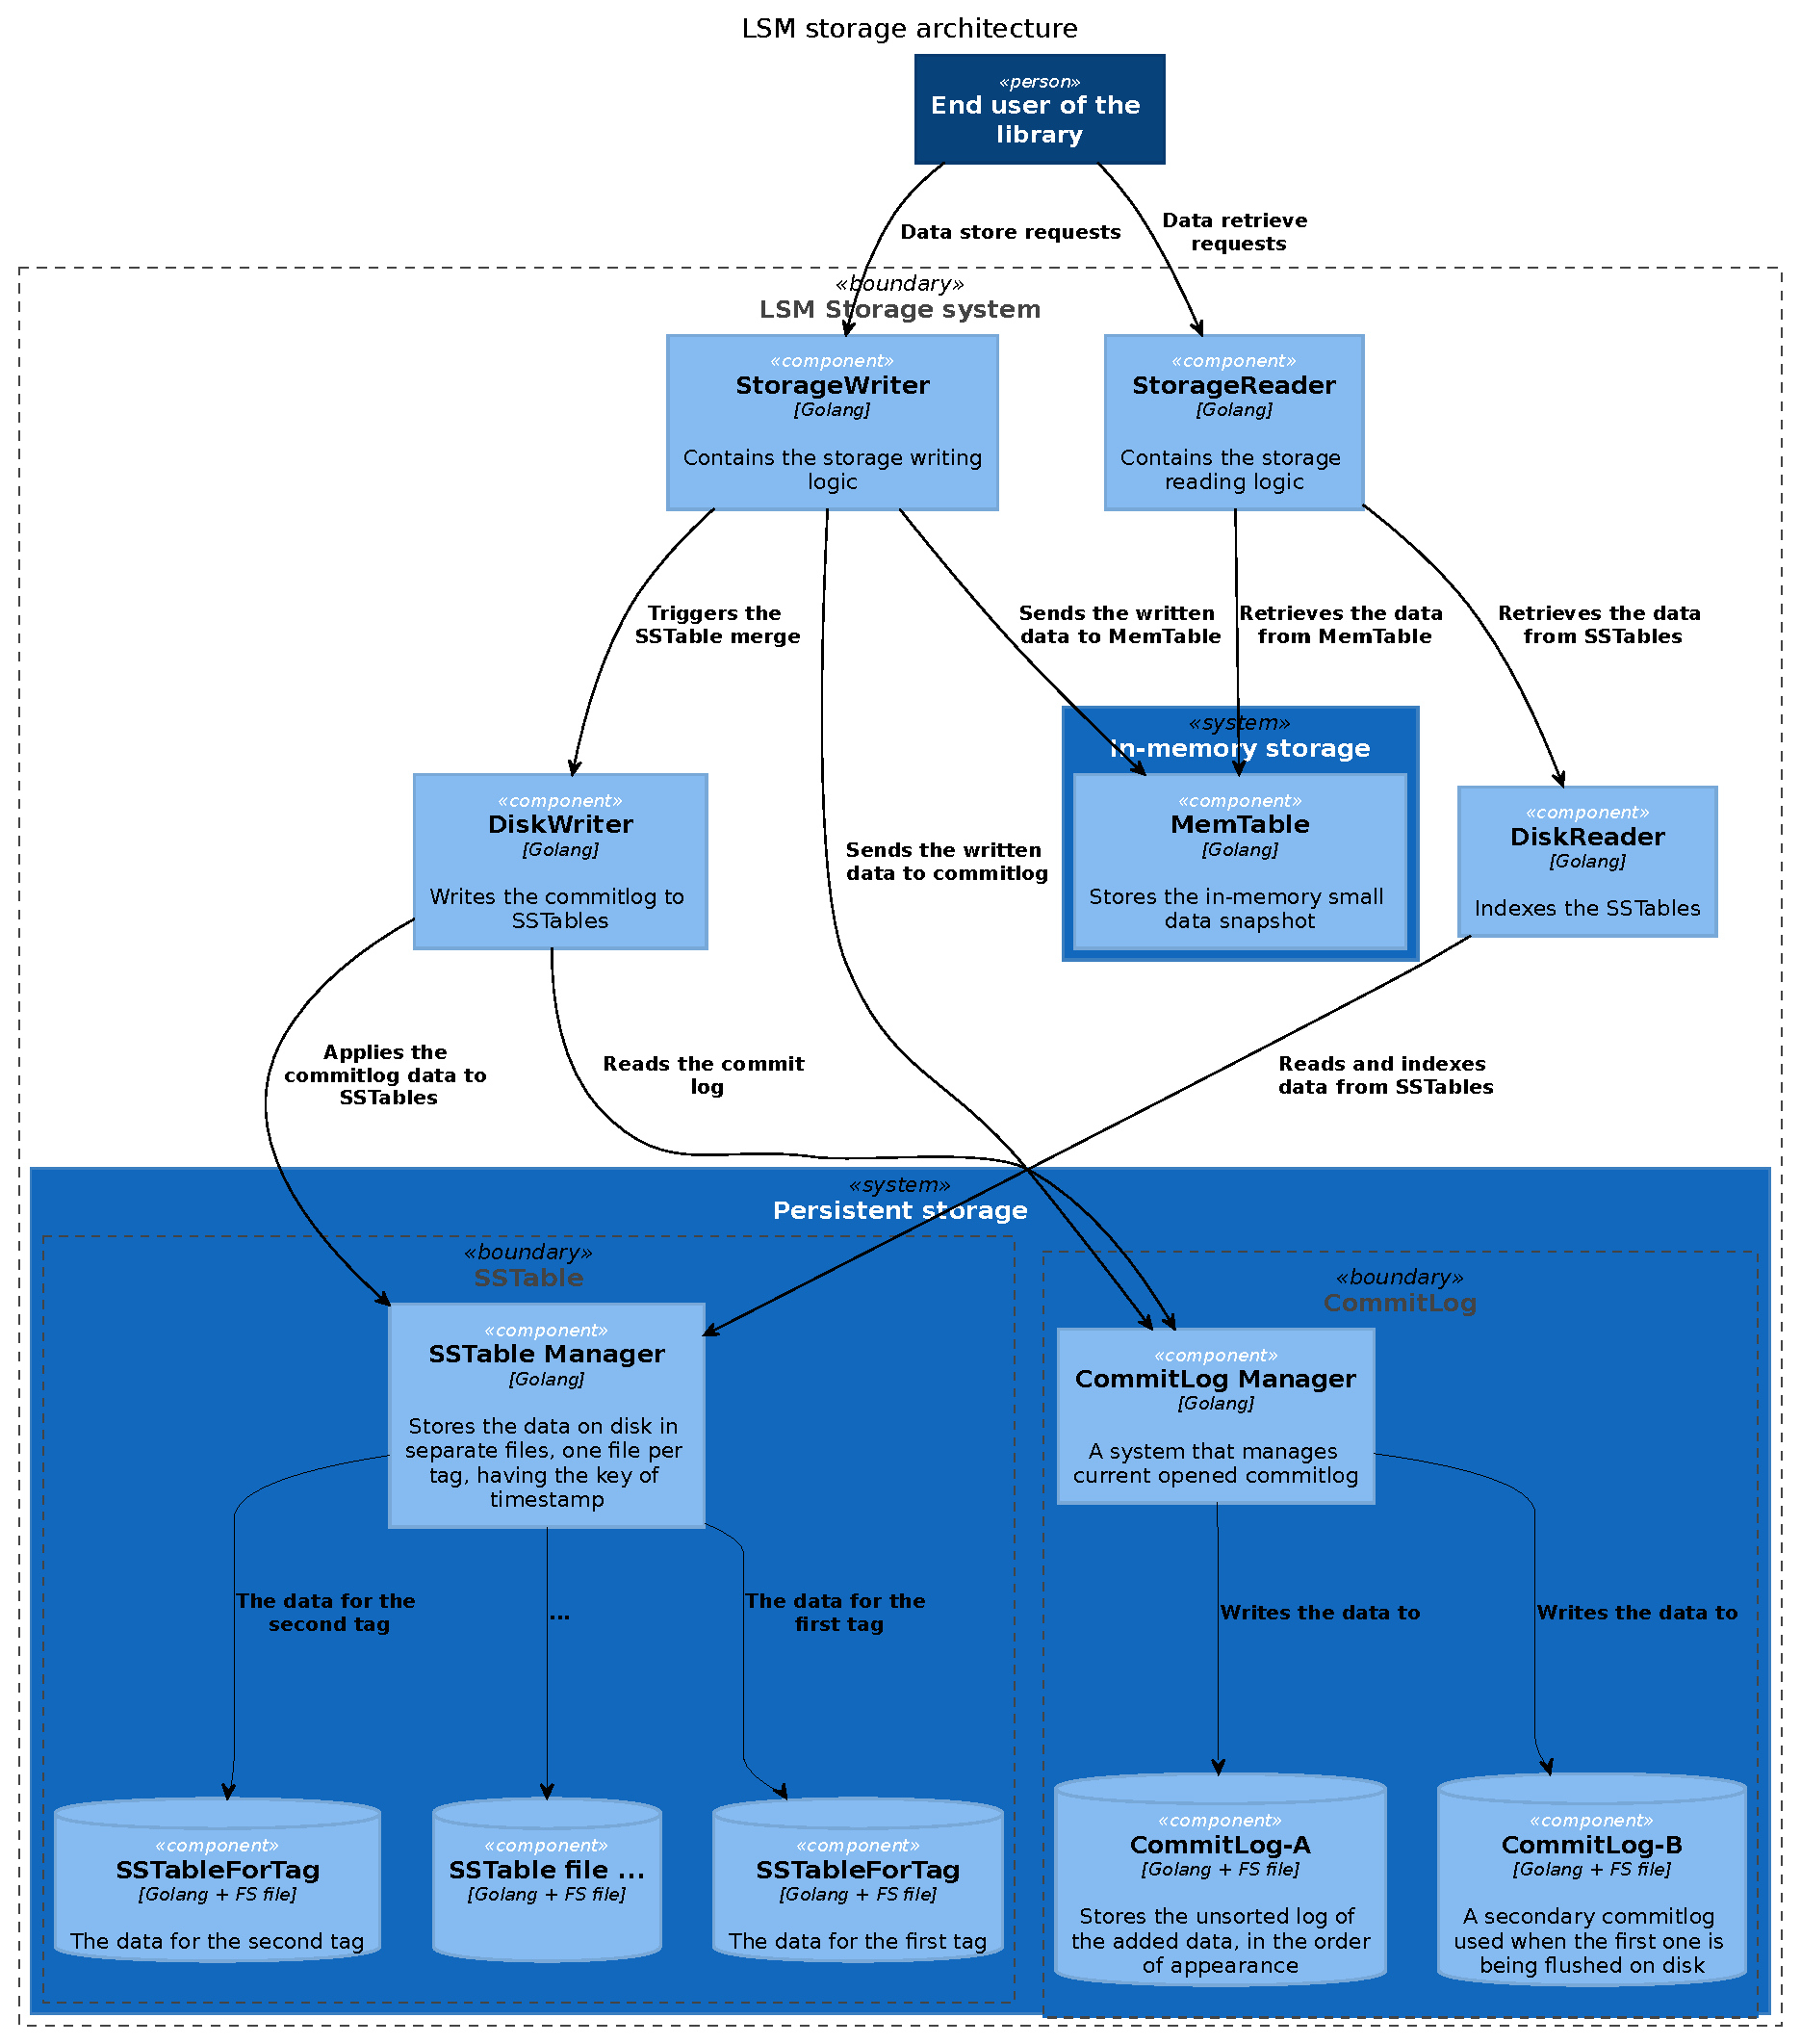
\includegraphics[width=\textwidth,keepaspectratio]{figures/golsm-arch.eps}
\caption{Архитектура библиотеки GoLSM.} \label{fig2}
\end{figure}

Поскольку эта библиотека изначально разрабатывалась для определенной предметной области и конкретного использования, у нее есть ряд ограничений. Например, у неё нет функций для удаления данных; вместо этого предполагается сохранить измерение с определенной датой истечения срока действия, после чего данные будут автоматически удалены в процессе уплотнения. Данные, которые хранятся с помощью GoLSM, должны состоять из одного или нескольких измерений; каждое измерение представлено именем тега, которое может быть идентификатором датчика или измерительного устройства, отметкой времени (origin), которая является отметкой, когда измерение было записано, и непосредственно значением измерения, которое сохраняется в виде массива байтов. Этот массив байтов может различаться по размеру, что усложняет процедуру сохранения каждого измерения.

Как видно из рисунка, система хранения состоит из двух уровней: уровня в памяти и уровня постоянного хранения. Уровень в памяти основан на реализации B-дерева от Google ~\cite{btree_google}. Он хранит небольшую часть данных настраиваемого размера. Уровень хранения состоит из диспетчера журналов фиксации и диспетчера SSTable. Диспетчер журнала фиксации поддерживает два файла журнала фиксации; в то время как один используется для записи текущих данных, другой используется для добавления ранее записанных данных в файлы SSTable, которыми управляет SSTable Manager. Каждый файл SSTable содержит один тэг, а также специальный индекс в памяти, который также основан на B-дереве. Этот индекс используется для ускорения извлечения данных из SSTable, когда запрошенный временной диапазон больше, чем то, что хранится на уровне в памяти.